\chapter{Introduction}\label{chapter1}

\lhead[\small\thepage\quad Chapter I]{}

%~ \vspace{-.3cm}

Among the early technologies, metallurgy holds a special place. It is a success story of human endeavour to control, manipulate and transform materials into relatively more durable and efficacious forms.~History of metal technology is replete with examples of new ventures in the field of metallurgy. In India, the mastery in metal casting techniques including the complex \textit{`cire perdue'} process in the $3^{\rm rd}$ millennium BCE is perceptible in the Harappan dancing girl and the Daimabad bronzes. The heavy tools and implements of the Copper Hoards in the Gangetic Plains in \textit{circa} 2500-1500 BCE or may be somewhat earlier also illustrate metallurgical skill of the metal workers in copper utilization. In the subsequent era, a hitherto unparalleled metallurgical expertise was mastered by ancient metal workers in extraction and forging of iron and distillation of metallic zinc.

Pure zinc could not be extracted in Europe even up to the 19th century, while use of metallic zinc in India can be traced back to the $4^{\rm th}$ -$3^{\rm rd}$ centuries BCE. Zinc production had reached almost industrial level in India by the $12^{\rm th}$ - $13^{\rm th}$ centuries CE. It was produced through distillation at an industrial scale as indicated by the heaps of zinc retorts found in the Zawar region of Rajasthan. Sizably large scale production of zinc continued for several centuries. Thus India may be given the credit of being the first country to master the complex technique to extract pure metallic zinc almost on an industrial scale by an indigenously developed distillation technique.

\newpage

The ingenuity and the innovative spirit of metal workers are also evidenced in the techniques of manufacturing of iron and steel at early date. This is fully borne out by the records of foreign travellers and historians who visited India in the past from time to time. For instance, Herodotus mentions iron arrowheads being used by the fighting army in the battle of Thermopylae in the 5th century BCE. Around the same time, Ktesias gratefully acknowledged the gift of swords of Indian steel made to him by the king and his mother at the Persian court. Quintus Curtis records that in North-western India, Alexander was presented with 100 talents of highly prized Indian steel in the form of ingots along with gold dust and other precious items in 326 BCE as a tribute. Arrian has also mentioned about import of Indian iron and steel into the Abyssinian ports. These Greek and Roman records thus bear a testimony to the importance of iron and steel produced in India and also to the fact that it was in great demand and prized in the ancient world civilizations because of its special quality. It was being exported to various parts of the world. Indian iron indeed appears to be a valuable commodity in the ancient times. Thus Indian iron was a commodity worth presenting to a monarch or other dignitaries way back in the $5^{\rm th}$ - $4^{\rm th}$ century BCE! 

In the following centuries iron technology grew manifolds, the mastery of the craft exhibits itself in the form of colossal structures like the seven-ton iron pillar at Delhi ($4^{\rm th}$ - $5^{\rm th}$ centuries CE). It has withstood the ravages of time for centuries. The technique developed by early iron workers was such that either it slowed down the rusting significantly or it almost stopped it once the oxide layer was formed. This property of rust resistance made Late Prof. T.R. Ananthraman, an eminent metallurgist of modern India, refer to Delhi Iron Pillar as the ‘Rustless Wonder of the World’. Equally significant in this regard are the large beams at the Sun temple at Konark that date back to the $9^{\rm th}$ -$10^{\rm th}$ century. The iron pillar at Dhar in central India is another iron master piece belonging to the $10^{\rm th}$ -$11^{\rm th}$ century. Besides the quality of rust resistance, these examples testify to the mastery in forging of colossal structures involving production and use of large quantity of iron having uniform properties. This in turn, also testifies to the presence of a well-organised production system capable of turning out tonnes of uniformly similar metallic iron during the early centuries of the Common Era. Forge-welding tons of iron with seamless precision is by no means a small achievement.  Little wonder that the skill and the expertise could easily be exploited subsequently by the state machinery during the medieval times for manufacturing weapons, especially cannons that adorn several important buildings today.

It may be interesting to underline the fact here that the British were surprised to see the high quality of iron and steel being produced in the traditional Indian iron workshops. They tested and rated highly the traditional Indian iron. The British engineers found it to be more suitable and strong for constructing bridges etc. than iron produced in their own production units. An important example in the case is the famous `tubular bridge' built in the early parts of the $19^{\rm th}$ century across the Menai Straits in the United Kingdom. It is categorically stated, ``...its (iron's) superiority is so marked, that at the time when the Britannia tubular bridge across the Menai Straits was under construction preference was given to the use of iron produced in India" (T.H.D. La Touché 1918). It has also been recorded that 50 tonnes of Indian steel have been used in construction of the famous London Bridge. This proves beyond doubt that traditional Indian iron and steel was superior to the pre-modern European steel. Indigenous iron was being imported from India by the British in $19^{\rm th}$ century for using it at strategically important points in iron structures like the London Bridge. The famous wootz steel is modified form of \textit{ukku} of Telugu language. Wootz, a very special kind of high carbon crucible steel, generally known as Damascus steel till recently was originally produced in India at around the beginning of the Common Era, or maybe even earlier as shown by recent excavations of megalithic sites like Kodumanal yielding evidence of steel making with crucibles, furnaces, slag, refractory material as early as 4th- 3rd century BCE (Rajan 2015: 65-79). The metallurgy of this enigmatic crucible steel making is still a subject of research among modern metallurgists. Several efforts have been made to reproduce high carbon steel with typical `watering pattern' though without much success. \textit{Wootz} was being exported to the outside world through various important ports of the ancient times. Presence of the `damascened' swords and daggers in so many important collections in different parts of the world is sufficient to prove both its significance as well as the scale of its production and its extensive distribution at a fairly early date. These facts have hardly been researched and brought to the notice in the publications on history of metallurgy (of iron). Despite the glorious past of Indian iron technology, volumes dealing with history of metallurgy do not have much to say about history of iron and steel in India.

The history of iron technology of Mesopotamia, the Greco-Roman world, Africa, China etc. are fairly well documented and hence better known to students of history of technology. One is amazed at the inadequacy of researches on Indian iron and steel. It is, therefore high time that an authentic history of iron technology in India covering its diverse aspects is produced. Indian contribution to this technology needs to be explored and given its due place in a global perspective of history of science and technology. The present volume is an attempt to present a comprehensive history of Indian iron and steel up to pre-modern times.

Reconstructing a comprehensive history of iron technology in India is indeed a difficult task.~In India there is a lack of systematic\break documentation of different practices. The oral tradition of knowledge transmission and the frequent destructions of manuscripts at educational centres by invaders in the early centuries of the medieval period have led to this vacuum.~Centres of knowledge such as those at Taxila, Nalanda, Vikramshila and private collections housed thousands of books in form of manuscripts. But the libraries of ancient times were frequently vandalized leading to an irreversible and permanent loss of scientific knowledge that existed in India.

There is very little knowledge available on the scientific basis of Indian metallurgy. There could be two reasons for it. Firstly, metallurgy was a practical skill mostly in the hands of a group of craftsman living in remote areas rich in ores and forests for charcoal as a source of energy. These craftsmen had little contact with the elite class of scholars. Secondly, possibly there existed a theoretical basis for the craft but the formulations have got lost in the course of time. It is improbable that high standards of metal technology and mastery - as illustrated by the examples mentioned above - could have been achieved without a proper scientific basis. Stray references to texts on iron metallurgy prove this point beyond doubt. This also dispels the notion that these skills were confined to a class or a caste based reservation and other restrictions associated with it. At least this must have been so at the initial stages. It is a different matter that metallurgy as a much specialised skill came to be associated with indigenous  groups of people and who got identified with it subsequently. It became the vocation of communities which were forest dwellers, may be for practical reasons like proximity to raw material. Later on such social groups were segregated and got identified with their vocations like iron working. They developed a social and cultural system of their own. It is this distant ethnic group that possesses some knowledge about iron working till date. They somehow carry the legacy of iron working. Whatever little remains with them today, need to be preserved and documented lest it gets lost forever.

The present volume on History of Science and Technology in India proposes to examine various dimensions of iron technology in India-right from its beginning to the stage of its development and the zenith it achieved, to its eventual decline after industrialization. It also proposes to look into the causes of its decline. Through a critical evaluation of sources, many of them not tapped so far, it may be possible to bring out several hitherto unknown or half known facets of history of iron technology in India. The book proposes to cover a long period of history spanning over several millennia - from emergence of iron in the second millennium BCE to the present day survival of the tradition. Though efforts have been made to collect as much information as possible up to the British period, at times the treatment of the subject may not be as comprehensive due to unavailability of necessary archival material.

Recent archaeological discoveries have attributed the first emergence of iron to copper-using societies in different parts of the subcontinent. The earlier contention of diffusion of iron has been questioned in light of new discoveries. We are faced with several questions that demand attention. How and under what circumstances metallurgy originated and evolved? Whether technology of iron was obtained through outside contacts or whether it evolved out of the existing knowledge of metal craft? In which part of the subcontinent did iron first appear? How did the metallurgy of iron develop? What are the stages of its development? Why is it that despite several attempts it has not been possible for modern metallurgists to unravel the mystery of wootz steel forging techniques? When was the impact of iron felt and why was it so slow to reflect itself in socio-economic milieu? What was the pattern of adaptation of iron technology in the early society? The interface of technology and society is yet to be examined and evaluated in all its dimensions. The causes responsible for the decline of a flourishing iron industry in India have to be looked into. The present study proposes to address such unresolved issues related to early Indian iron technology (See, figures~{\ref{chapter1-fig001}}, \ref{chapter1-fig002} and \ref{chapter1-fig004} for early Iron Age sites and Fig.~\ref{chapter1-fig003} for pre-industrial sites). 

With new researches in archaeo-metallurgy and radiocarbon dating of recently excavated sites in India, one needs to take a fresh look at the issue of origin of iron in India. The other important issue that needs attention is the role of iron in cultural changes. We need to review and interface productivity, technology advancement, and its pattern of adaptation by society at nodal points of history. The status of metallurgy at various stages of development has to be defined and its adaptation in proper cultural context has to be studied. This has to be attempted at several stages of cultural growth. Iron metallurgy had a prolonged incubation period. Its impact on society was indeed slow. All this should be examined in detail to be able to address the unanswered questions that keep coming up every now and again. 

As noted earlier, iron production was sufficiently developed in India by the $4^{\rm th}$-$5^{\rm th}$ century CE. It was organized enough to produce colossal structures like the Delhi iron pillar. Wootz steel became an important and prized commodity all over the ancient world. Metallurgy in India during this period attained an unparalleled status. It is important to delve deep into its production and distribution mechanisms. Metallurgical developments and innovations through the medieval and the British periods are recorded in the contemporary writings and they may provide valuable insights into the subject. All this has to be examined at various nodal points of cultural development – beginning from the early-medieval and medieval times and even beyond, up to pre-modern age. As the iron technology attains maturity, it manifests unparalleled mastery. One wonders as to how it found its way into the world market. The dynamics of distribution and dispersal of commodities, especially a prized commodity like Indian steel needs to be probed.

Right from ancient times, India carried out over land and sea trade with West Asia, China, South-East Asia and also Africa. Trade with the Gulf region has been frequently mentioned in various texts. A large number of port towns from Sind (Bambhore) in present day Pakistan through those in Central–Western parts of India (Gulf of Cambay, Broach) right up to the peninsular India (Coromandel, Cochin, Kaveripattanam etc.) were busy ports. Puranas make frequent references to sea–faring traders. \textit{Agnipurana} mentions that Soppora (Shurpârak), Vanga (Bengal), Anga (Bhagalpur in Bihar) were centres of steel making. The historian of medieval times, Idrisi, makes a specific reference to purchase of Indian steel swords. Even the Chinese scholar Chau Ju Kua ($8^{\rm th}$ century CE) talks of import of steel rods (ingots?) from India through the sea route during early medieval period. Indian ships brought back horses and exported copper, tin, lead and solid steel (ingots?), spices, drugs, cotton cloth, precious stones, timber, leather goods and other luxury items. In the early medieval ages, India carried out trade with Iran, Iraq (ancient Mesopotamia), Indonesia, and as mentioned above, with China. There are references of rich Indian traders living in Mesopotamia. India mostly received gold in return from many countries.

\vspace{-0.3cm}

\begin{figure}[H]
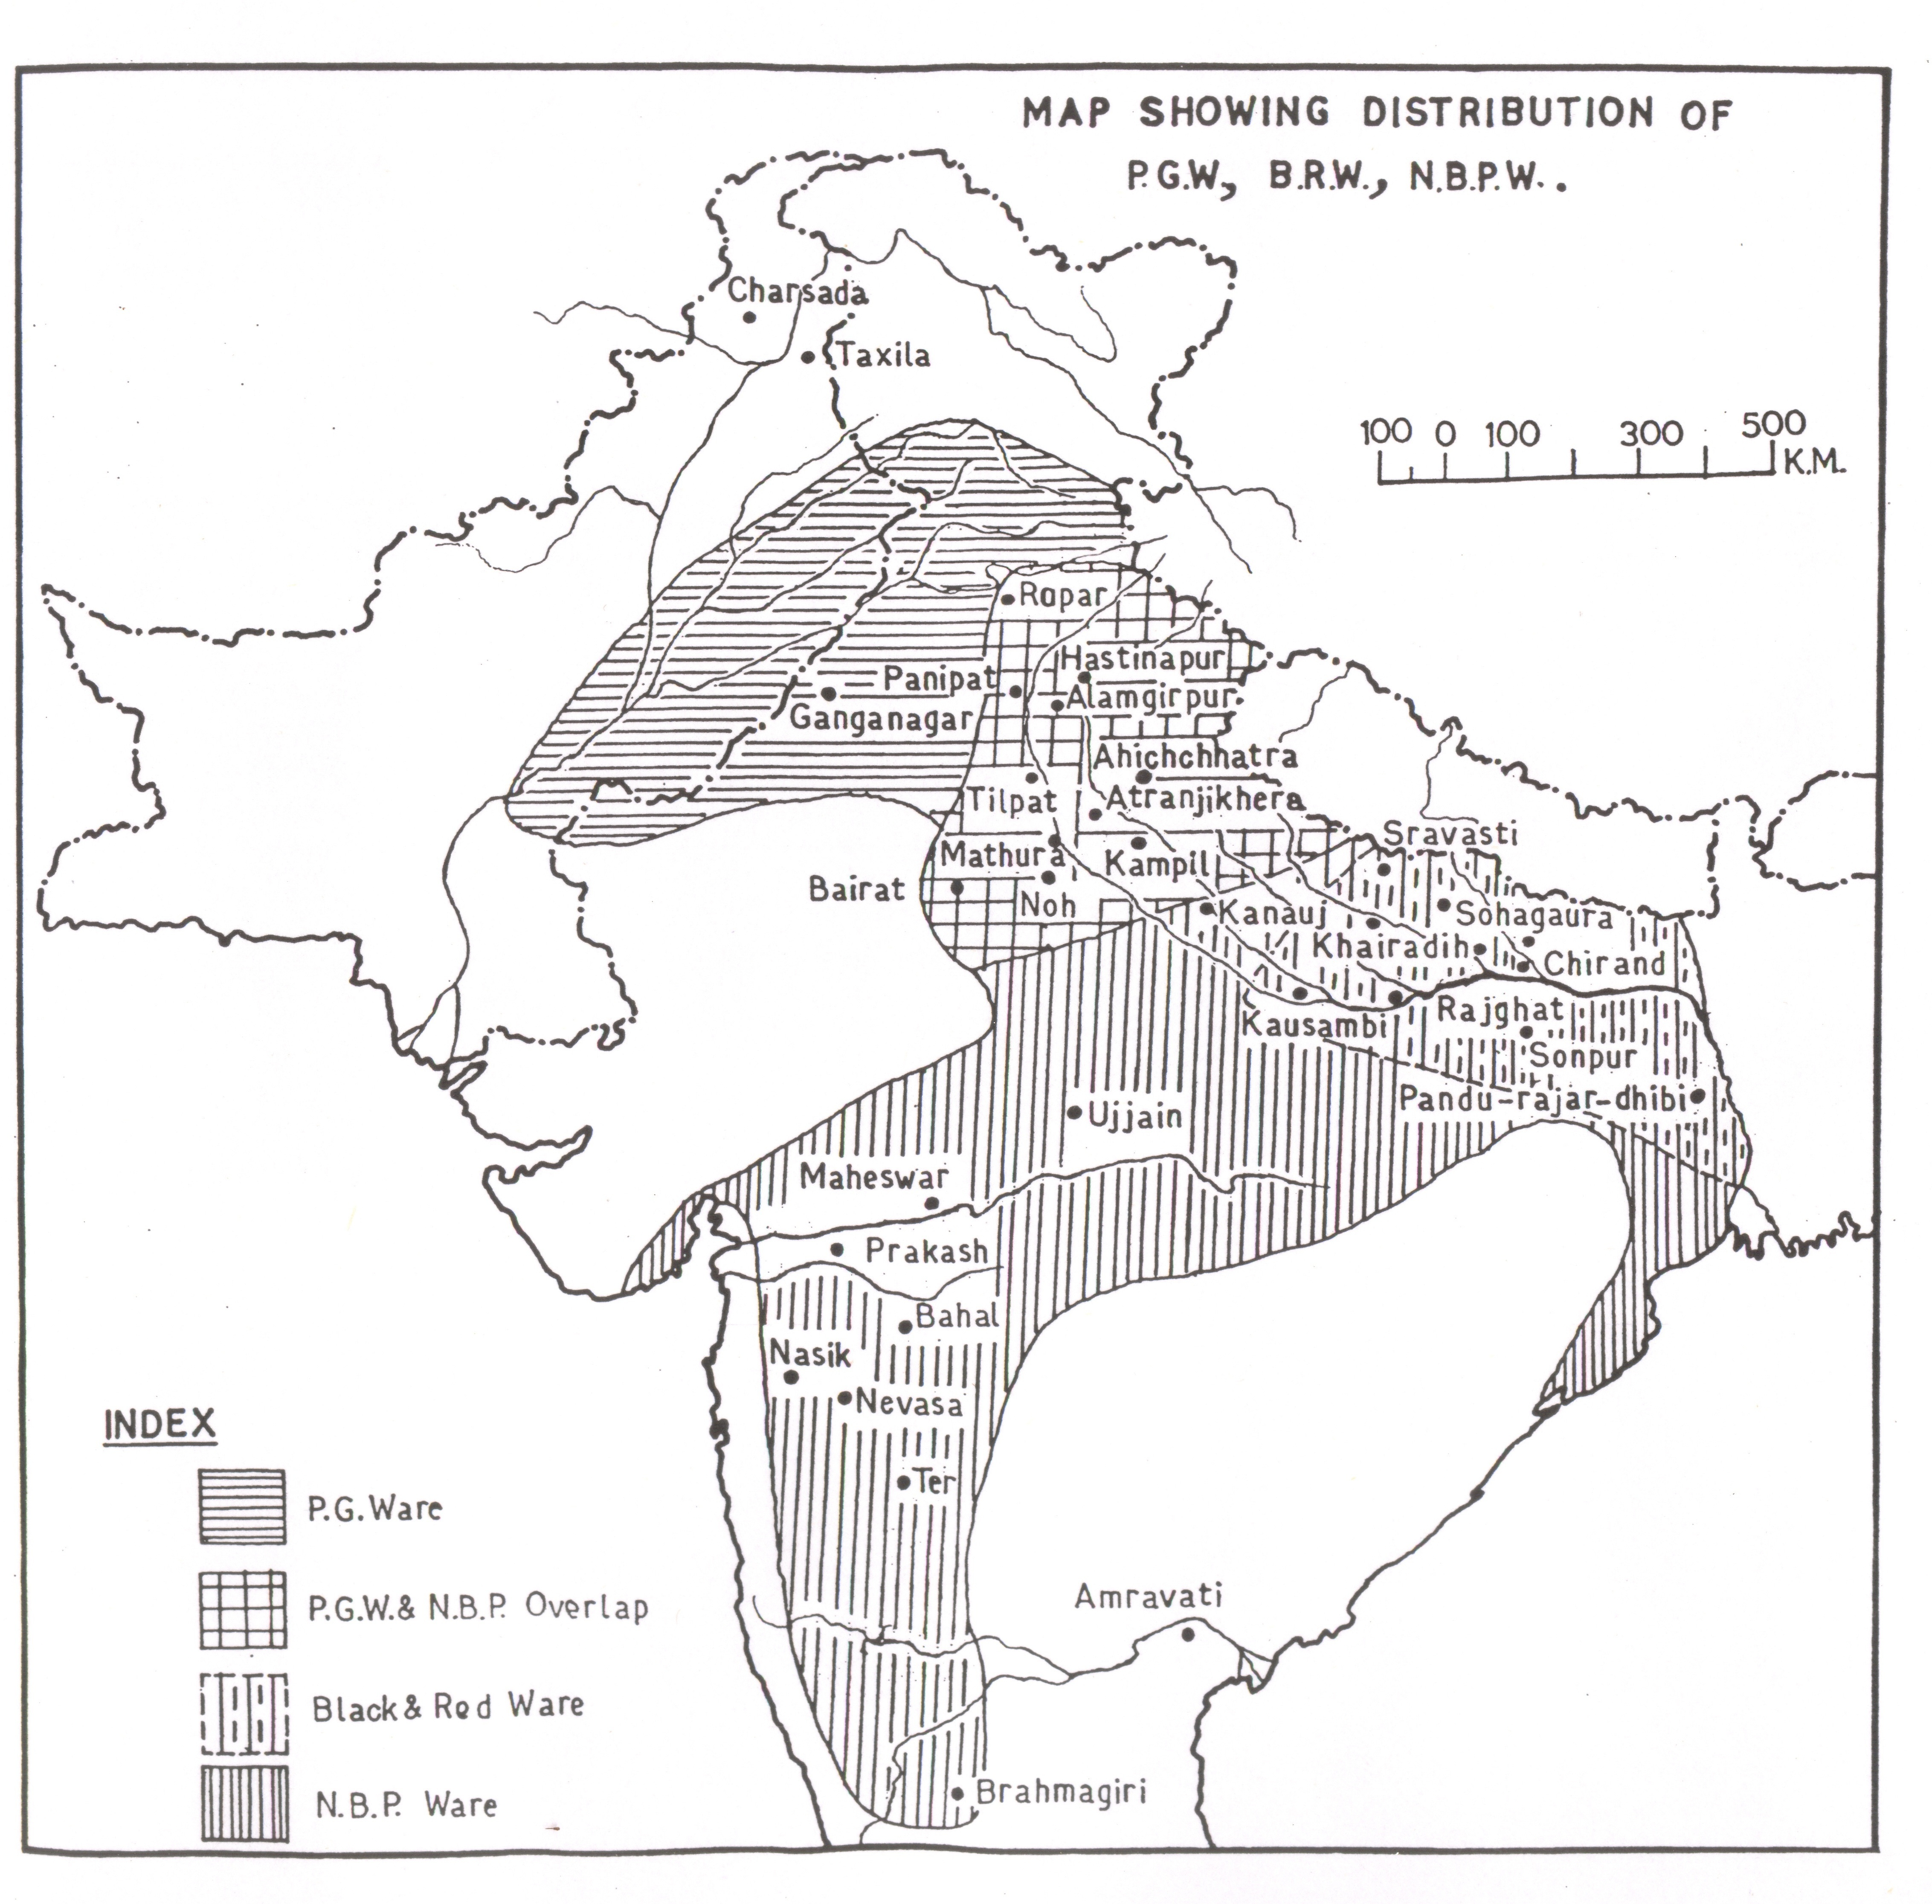
\includegraphics[scale=.5]{images/chapter-1/fig001.jpg}
\caption{\textit{Map showing distribution of P.G.W., B.R.W. and N.B.P.W.}}\label{chapter1-fig001}
\end{figure}

\newpage

\begin{figure}[H]
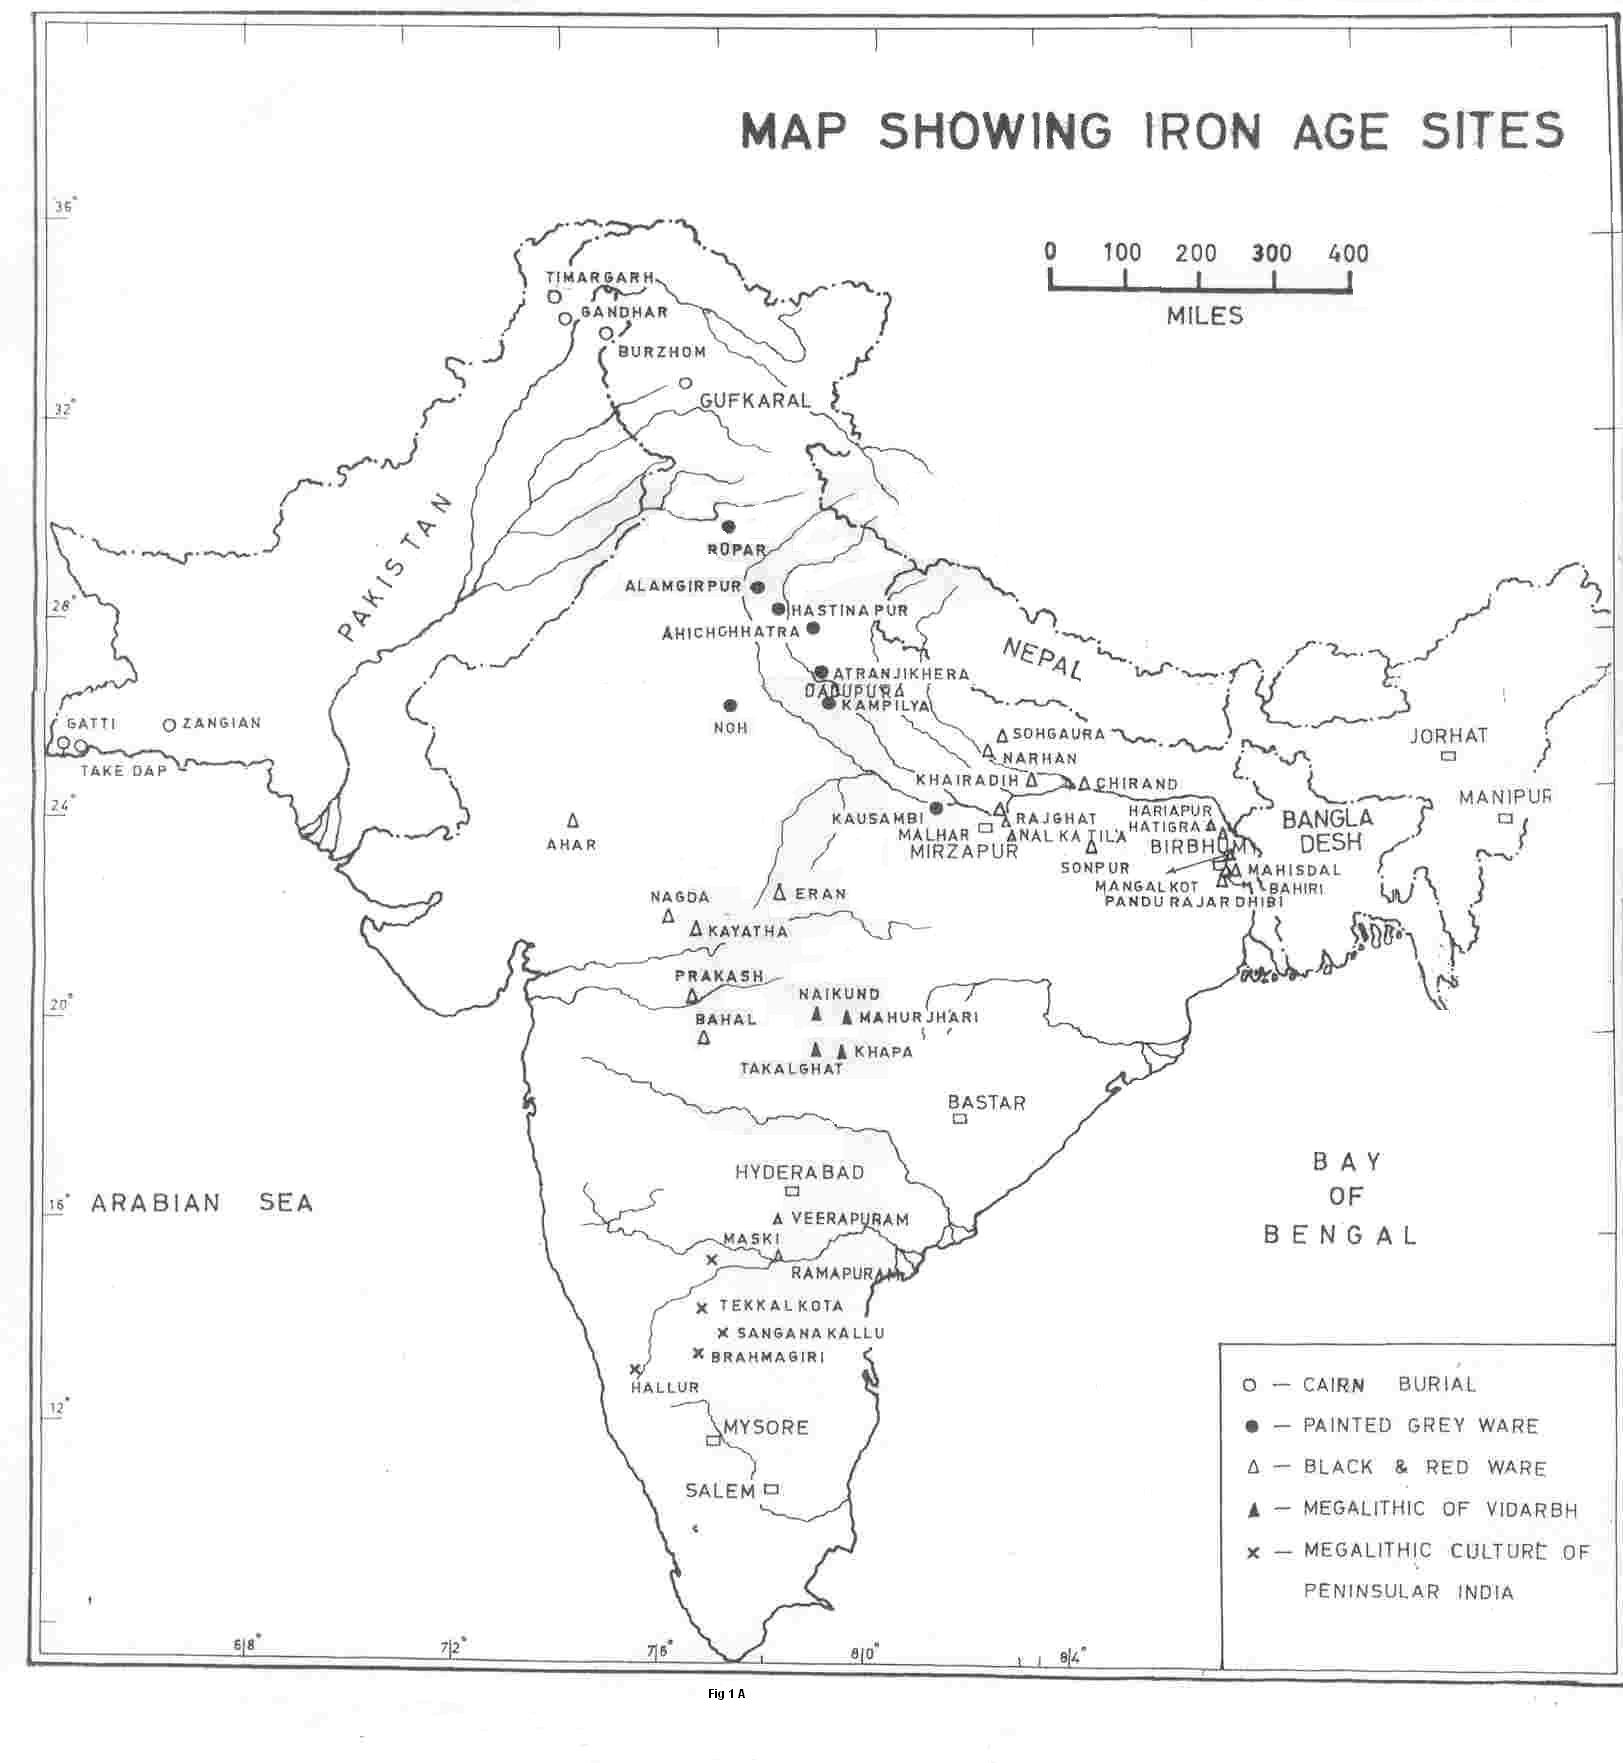
\includegraphics[scale=1.5]{images/chapter-1/fig002.jpg}
\caption{\textit{Different Zones of Iron Age Cultures of India}}\label{chapter1-fig002}
\end{figure}


\newpage

\begin{figure}[H]
\begin{center}
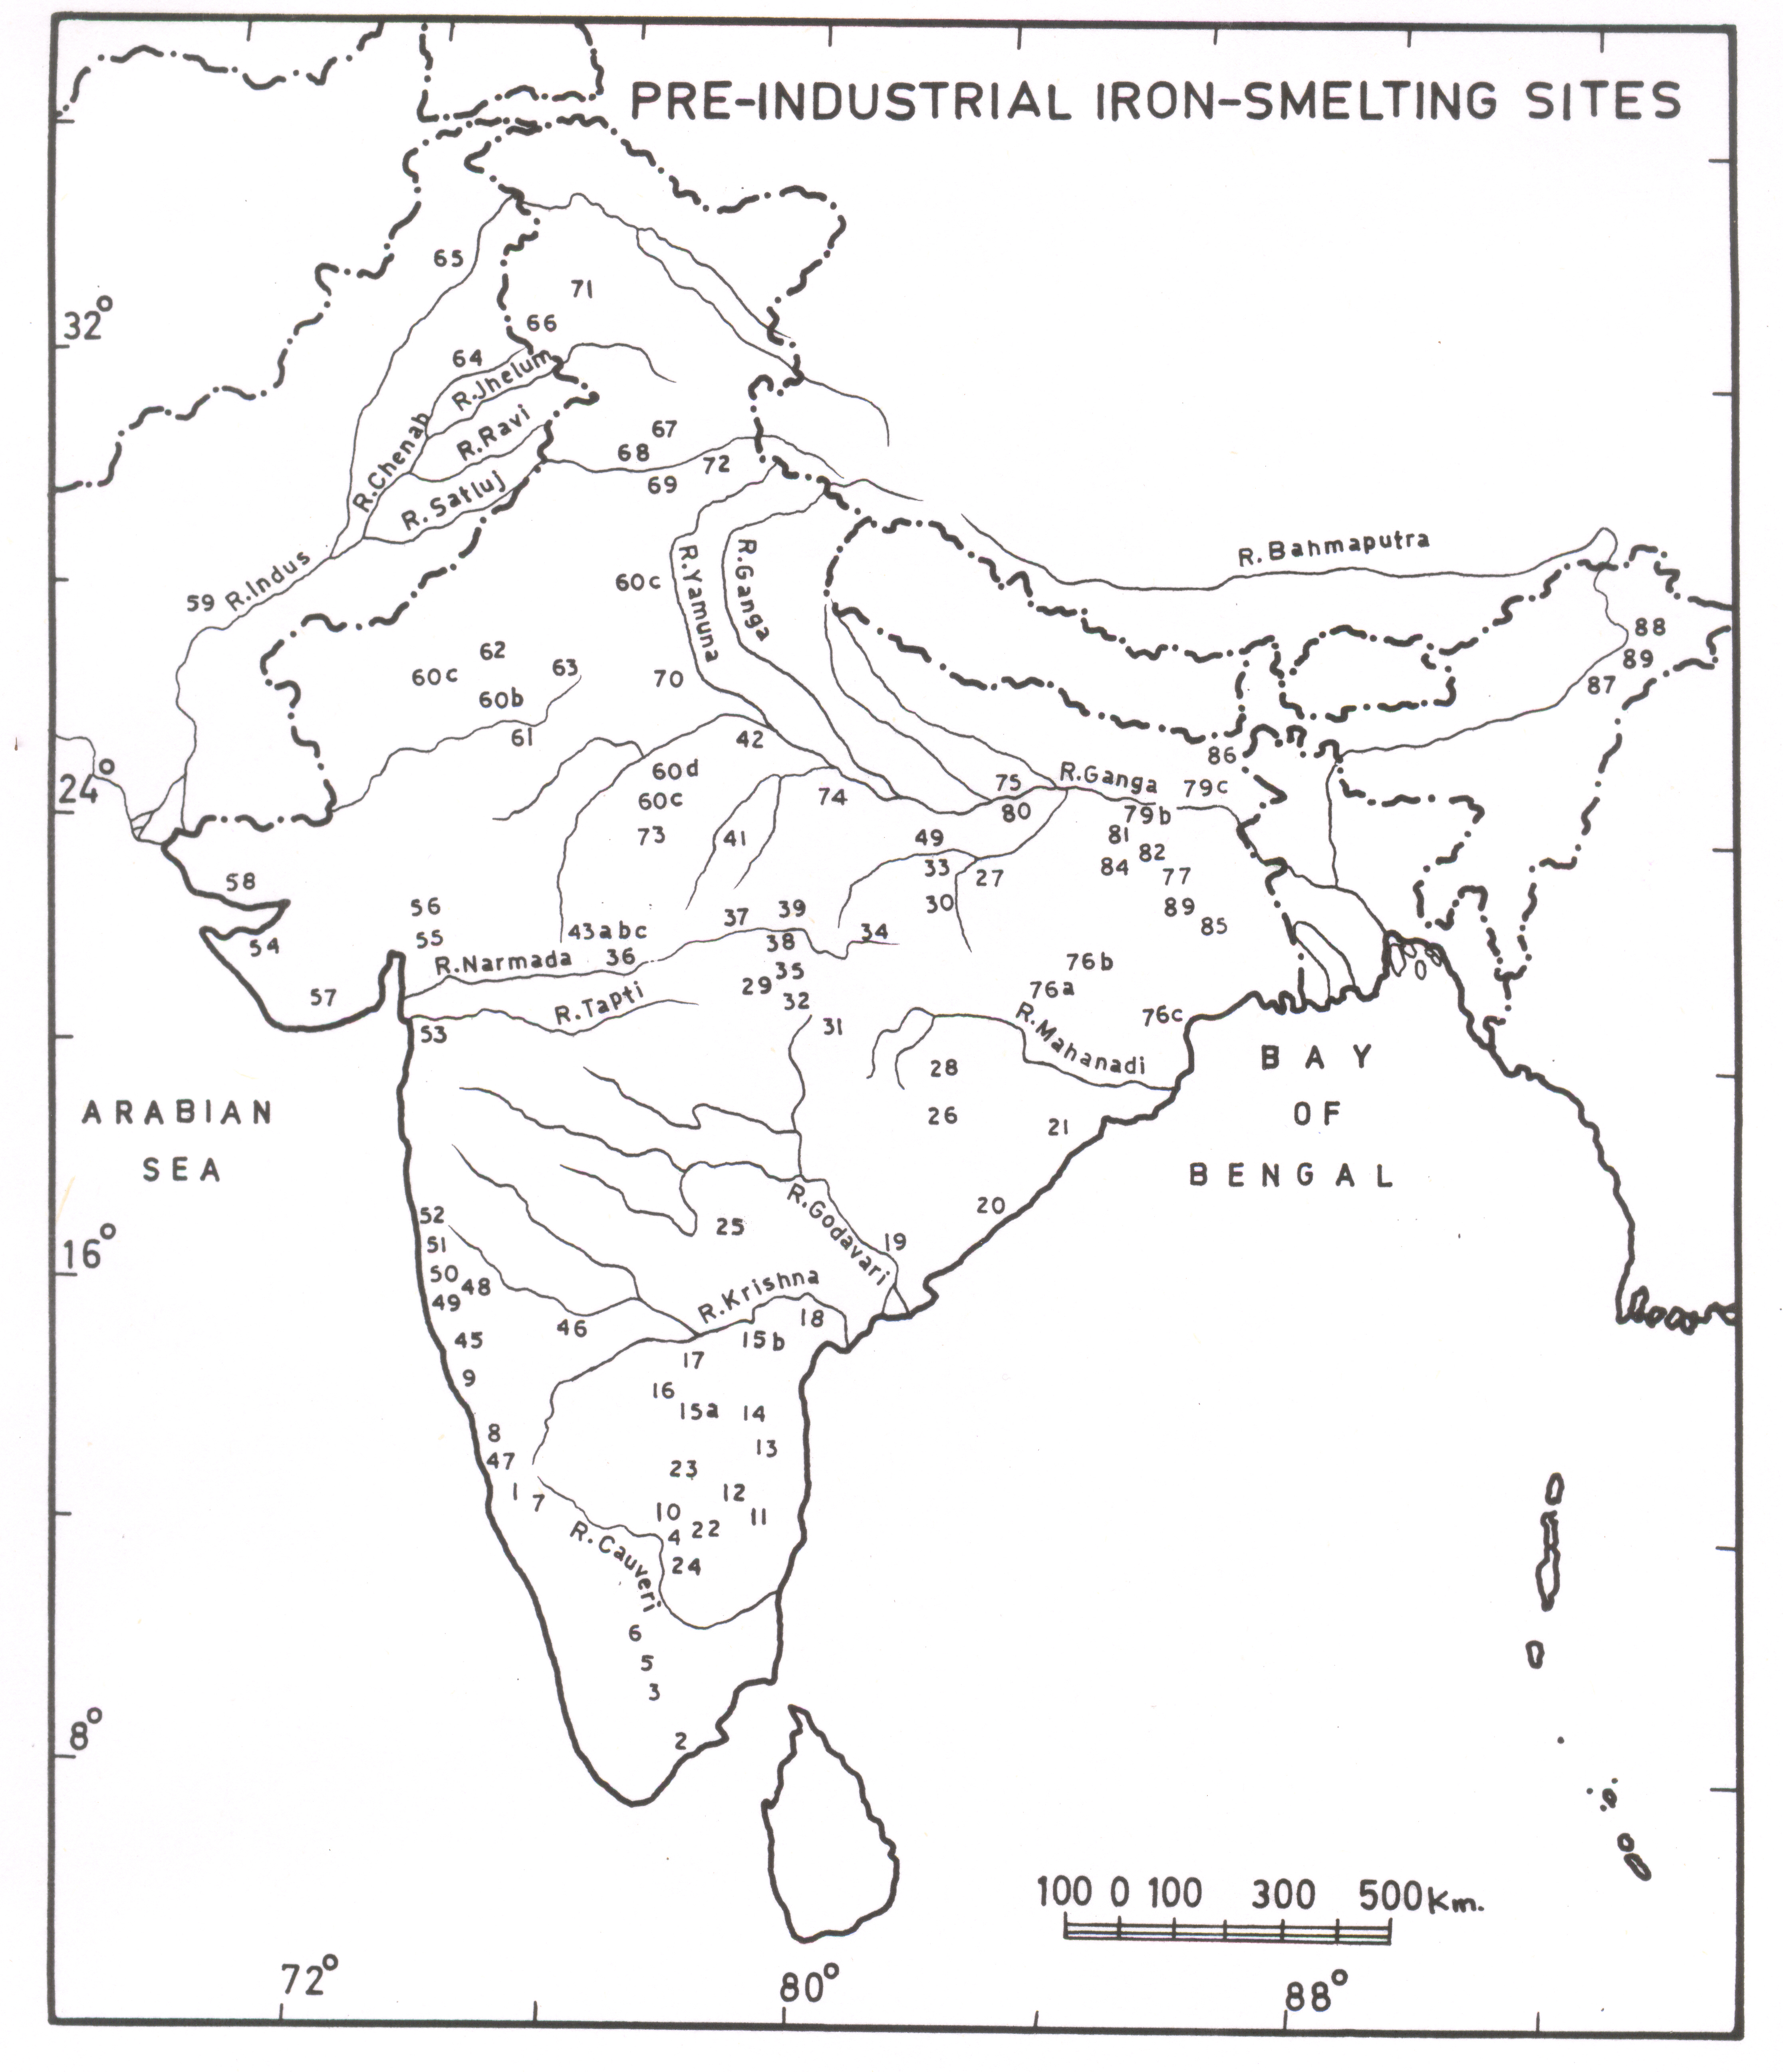
\includegraphics[scale=0.47]{images/chapter-1/fig003.jpg}
\caption{\textit{Distribution of pre-industrial iron working sites\\ (sites are numbered)}}\label{chapter1-fig003}
\end{center}
\end{figure}

\newpage

\begin{figure}[H]
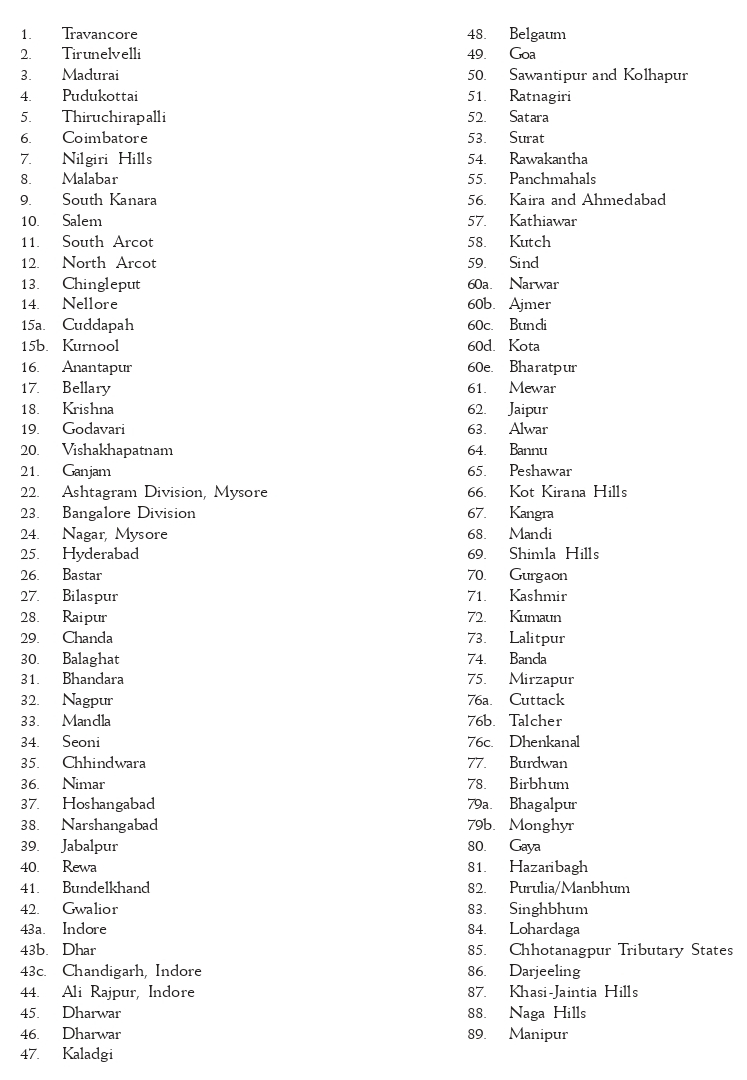
\includegraphics[scale=.7]{images/chapter-1/fig003a.jpg}
\caption*{\textit{Key to Fig. 3 (After Chakrabarti 1992 Fig. 13)}}\label{chapter1-fig003a}
\end{figure}

\newpage


\begin{figure}[H]
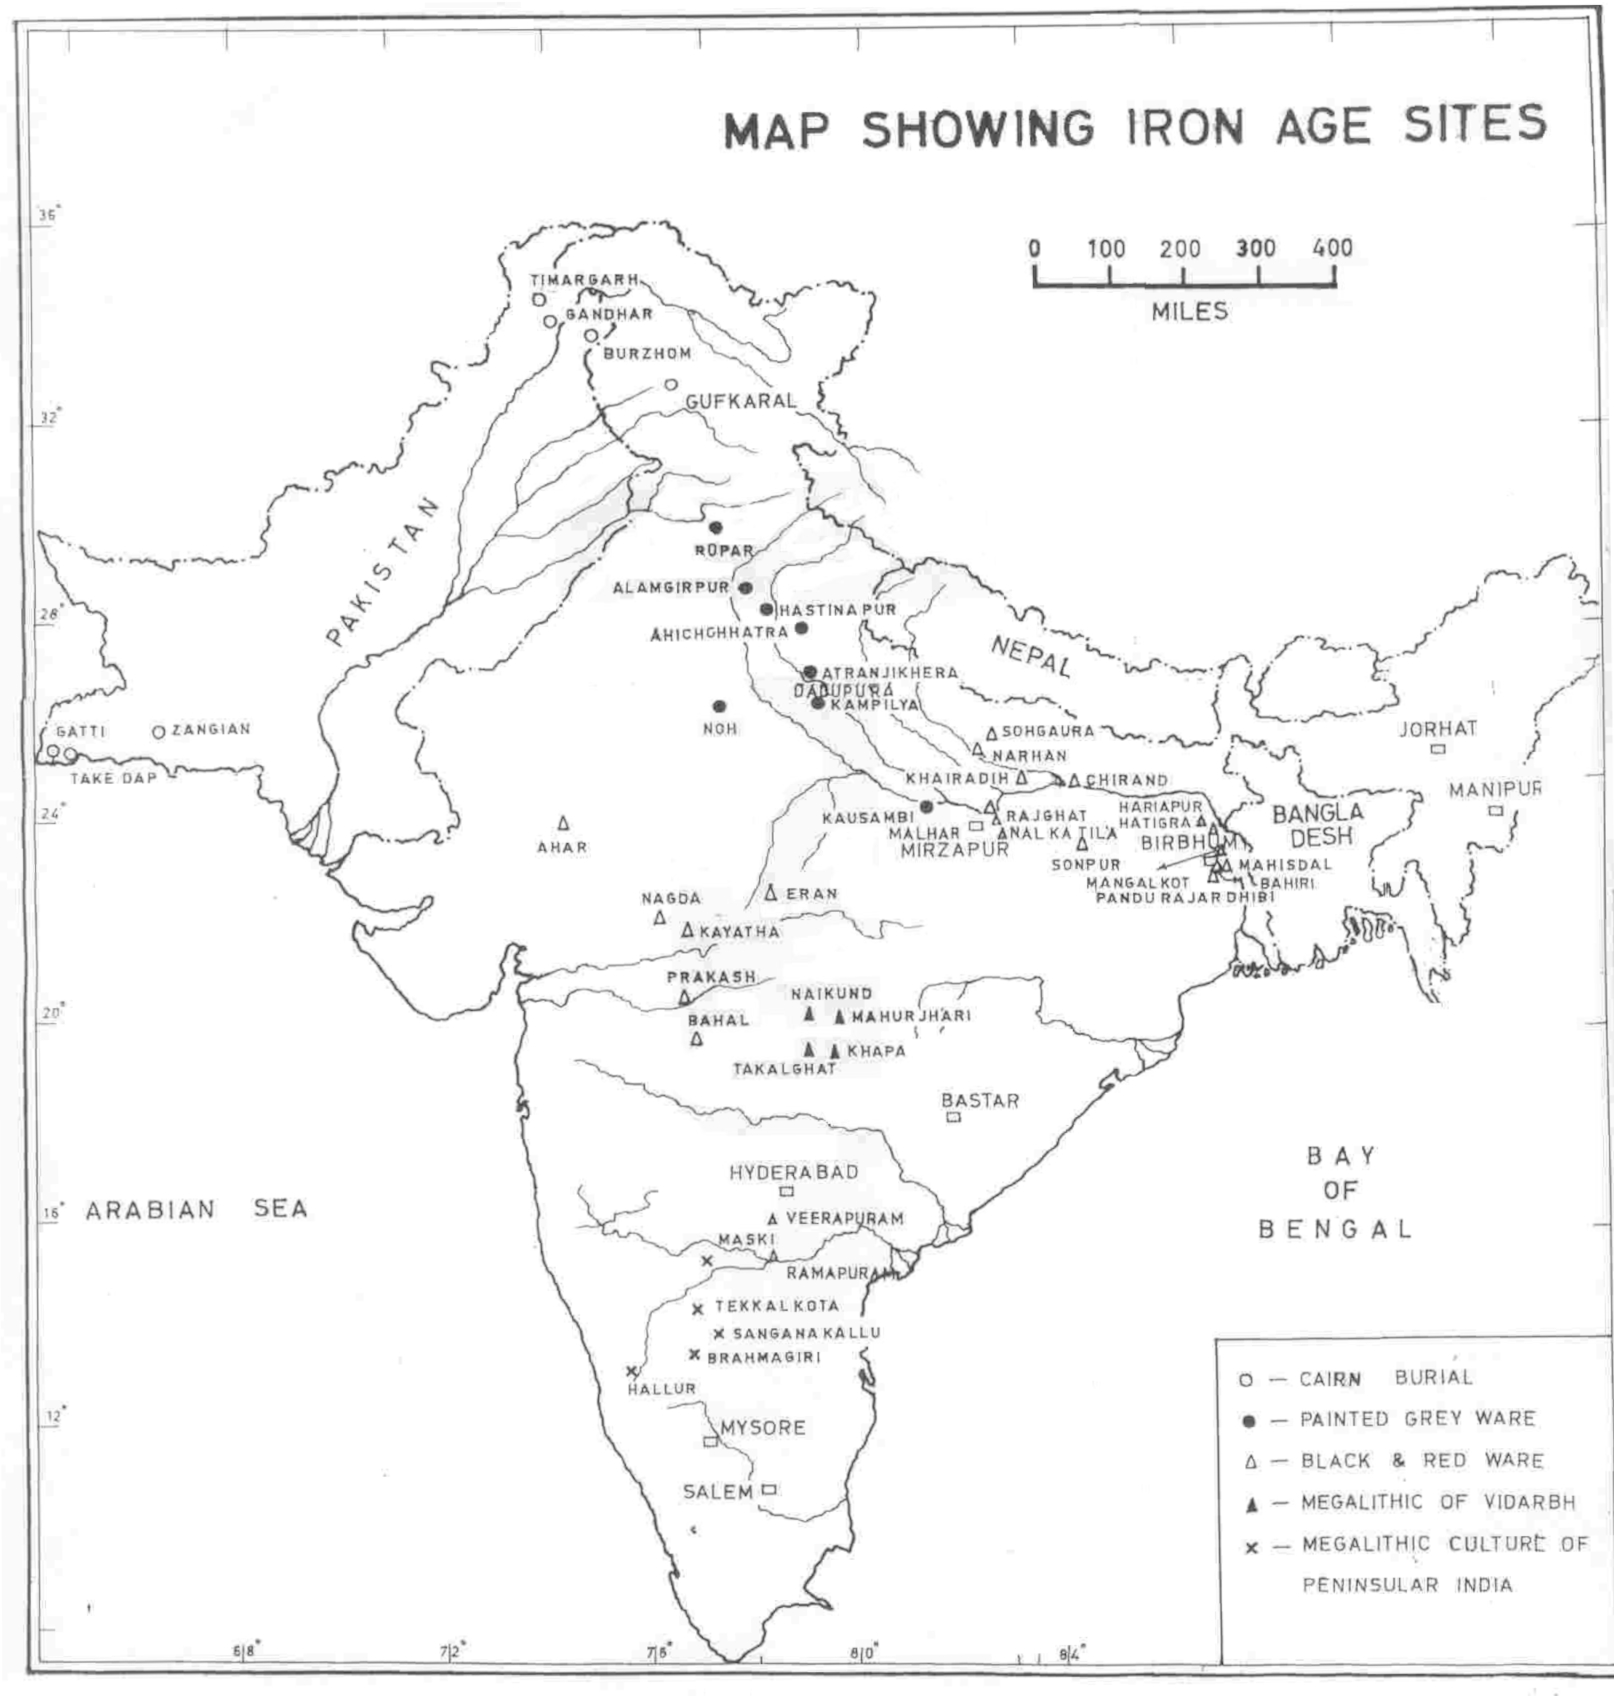
\includegraphics[scale=0.23]{images/chapter-1/fig004.jpg}
\caption{\textit{Map showing Iron Age sites}}\label{chapter1-fig004}
\end{figure}

%~ {\fontsize{6}{7}\selectfont\begin{longtable}{|p{.35cm}|p{1.5cm}|p{.35cm}|p{1.9cm}|}
%~ \caption{{\fontsize{6}{7}\selectfont Key to Fig. 3 (After Chakrabarti 1992 Fig. 13)}}\label{chapter1-fig004}\\

%~ \hline
%~ \endfirsthead
%~ \hline
%~ \endhead
%~ \hline
%~ \endfoot
%~ \endlastfoot
%~ 1 & Travancore & 48 & Belgaum\\\hline
%~ 2 & Tirunelvelli & 49 & Goa\\\hline
%~ 3 & Madurai & 50 & Sawantipur and Kolhapur\\\hline
%~ 4 & Pudukottai & 51 & Ratnagiri \\\hline
%~ 5 & Thiruchirapalli  & 52 & Satara \\\hline
%~ 6 & Coimbatore & 53 & Surat \\\hline
%~ 7 & Nilgiri Hills & 54 & Rawakantha \\\hline
%~ 8 & Malabar & 55 & Panchmahals  \\\hline
%~ 9 & South Kanara & 56 & Kaira and Ahmedabad \\\hline
%~ 10 & Salem & 57 & Kathiawar\\\hline
%~ 11 & South Arcot & 58 & Kutch\\\hline
%~ 12 & North Arcot & 59 & Sind\\\hline
%~ 13 & Chingleput & 60a & Narwar \\\hline
%~ 14 & Nellore & 60b & Ajmer\\\hline
%~ 15a & Cuddapah & 60c & Bundi \\\hline
%~ 15b & Kurnool & 60d & Kota\\\hline
%~ 16 & Anantapur & 60e & Bharatpur \\\hline
%~ 17 & Bellary & 61 & Mewar \\
%~ 18 & Krishna & 62 & Jaipur \\\hline
%~ 19 & Godavari & 63 & Alwar \\\hline
%~ 20 & Vishakhapatnam & 64 & Bannu \\\hline
%~ 21 & Ganjam & 65 & Peshawar\\\hline
%~ 22 & Ashtagram Division, Mysore  & 66 & Kot Kirana Hills\\\hline
%~ 23 & Bangalore Division & 67 & Kangra \\\hline
%~ 24 & Nagar, Mysore & 68 & Mandi \\\hline
%~ 25 & Hyderabad & 69 & Simla Hills\\\hline
%~ 26 & Bastar & 70 & Gurgaon \\\hline
%~ 27 & Bilaspur  & 71 & Kashmir\\\hline
%~ 28 & Raipur & 72 & Kumaun \\\hline
%~ 29 & Chanda  & 73 & Lalitpur \\\hline
%~ 30 & Balaghat & 74 & Banda\\\hline
%~ 31 & Bhandara & 75 & Mirzapur \\\hline
%~ 32 & Nagpur & 76a & Cuttack\\\hline
%~ 33 & Mandla & 76b & Talcher\\\hline
%~ 34 & Seoni  & 76c & Dhenkanal\\\hline
%~ 35 & Chhindwara  & 77 & Burdwan\\\hline
%~ 36 & Nimar & 78 & Birbhum\\\hline
%~ 37 & Hoshangabad  & 79a & Bhagalpur\\\hline
%~ 38 & Narshangabad & 79b & Monghyr\\\hline
%~ 39 & Jabalpur & 80 & Gaya\\\hline
%~ 40 & Rewa  & 81 & Hazaribagh\\\hline
%~ 41 & Bundelkhand  & 82 & Purulia/Manbhum\\\hline
%~ 42 & Gwalior & 83 & Singhbhum\\\hline
%~ 43a & Indore  & 84 & Lohardaga\\\hline
%~ 43b & Dhar  & 85 & Chhotanagpur Tributary\phantom{} States\\\hline
%~ 43c & Chandgarh, Indore  & 86 & Darjeeling\\\hline
%~ 44 & Ali Rajpur, Indore & 87 & Khasi-Jaintia Hills\\\hline
%~ 45 & Dharwar & 88 & Naga Hills\\\hline
%~ 46 & Dharwar & 89 & Manipur\\\hline
%~ 47 & Kaladgi &    &  \\\hline
%~ \end{longtable}}

\vspace{-.5cm}

Such well-established trade in this region must have provided incentive to iron and steel industry of India. As mentioned above, there were well-established port towns in ancient India that find mention in literature from time to time. Banbhore or Bambhore was a busy ancient port on the river Indus in Sind. It was located 40 km. east of Karachi - Periplus refers to it as Barbaricum and Ptolemy as Barbari. This was an active and busy port at least from the $1^{\rm st}$ to $13^{\rm th}$ century CE. Ancient ceramics from Syria, Susa and Iran have been found there. Likewise, Al Idrisi rated the Gulf of Cambay as a beautiful and the safest seaport. The writings of Istakhari and Ibn Haukal in 951 CE describe it as an important port. The latter has praised the swords made at Debal in Sind (HIED, I: 37). Al Masudi, also of the $10^{\rm th}$ century CE, and Al Beruni have mentioned Broach as an important port. It is the place where river Narmada meets the sea. Up to the $11^{\rm th}$ - $12^{\rm th}$ century CE, the Chinese and Arabs frequently visited the Indian ports. Although it has not been possible to get a detailed inventory of the commodities that were being traded in, but it is a fact that Sind, Gujarat, Kachch, Bengal, Bihar and Peninsular India were famous for their steel, especially for the highly acclaimed steel swords that they produced. There is every likelihood that steel must have been an important export item. Later on, as late as the British period, the indigenous iron and steel industry flourished. It has been studied, appreciated and criticized by the British engineers for its strengths and weaknesses. The sword of Tipu Sultan was an enigma and is almost like a legend today. However, the reasons of virtual disappearance and general decline of iron working in succeeding centuries need to be investigated. 

British engineers and geologists took pains to study Indian iron metallurgy. Any history of technology should incorporate observations made by experts on strengths and weakness of the indigenous system of iron working. The present volume attempts to undertake a rather difficult task of surveying a long span of history of iron technology in India. It spans through the issue of emergence of iron in the Indian subcontinent sometime in the $2^{\rm nd}$ millennium BCE and the process of metallurgical development through the centuries. At the same time there is also an attempt to take a look at the status of iron technology during the early medieval period. The history of iron technology has many facets within the period ranging from the Imperial Guptas to the mighty Moghuls. There were changes in the socio-political milieu during different cultural stages. Whether technological processes were influenced and affected by such upheavals of history is an issue that this book proposes to examine. 

It may be worth underlining an interesting fact that King Bhoja of Dhar composed a treatise on iron manufacturing in the $10^{\rm th}$ – $11^{\rm th}$ century CE. He even mentioned a couple of other texts, which had been composed earlier. It is significant indeed in view of the fact that it has always been believed that metallurgy in India was only a craft being practiced by the artisans. But presence of three-four treatises on such a complex technology sufficiently emphasises the importance of iron technology during the ancient times. It also demonstrates that iron had acquired the status of a full-fledged science by the $10^{\rm th}$ – $11^{\rm th}$ century CE or may be even earlier. It is unfortunate that these texts which could well have been like manuals on the subject for experts of that age have not been recovered so far. But it is certain that by the early mediaeval times iron technology had acquired the status of a scientific discipline that engaged the attention of scholars and well informed rulers who chose to write texts for the benefit of the interested readership of their times.

The medieval period was an age of expansion and consolidation of power on the one hand and of deconstruction of the basic structure of the Indian society on the other. The Mohammdan invasions in the $12^{\rm th}$ – $13^{\rm th}$ centuries CE had far-reaching consequences on Indian social system. They were not only devastating, but also brutal to the extent that entire populations were captured and made slaves. Qutubuddin Aibak's invasion of Gujarat (1195 CE) netted him twenty thousand slaves. Seven years later (1202 CE) he raided Kalinjar and ‘fifty thousand slaves were brought under chain' (Nizami, quoted by Habib 1984: 90). Firuz Tughluq enslaved twelve thousand artisans (1351-88). Under the Muslim law slaves were saleable. Barni describes slave market in Delhi. This practice must have adversely hit the Indian socio-economic set up, affecting the production mechanism of the contemporary society. However, Habib speaks of a decline in the slavery after 14th century due to ``availability of cheaper free labour in such crafts and professions..." created for the nobility. It was under such circumstances that villagers started fleeing their homes, \textit{en masse} leaving their professions and belongings behind. No doubt the exodus included artisan class also. The atrocities on hapless common men turned them into hopeless poor wretches fleeing for their lives. It is futile to talk of innovation, creativity, knowledge, and incentives in such a milieu. 

It was a period when several monumental edifices of the ancient times were demolished, including the iron pillar at Dhar, perhaps the tallest of its kind in the world. At the same time it was an age of reorganization of techno-cultural forces. The values seem to be redefined as evidenced in the production of such monumental structures. Instead of victory pillars and tributes to the deities and shrines, arms and armours assumed greater importance. The artisans were commissioned to produce weapons to their utmost capacity. This was needed to equip military forces for incessant wars that were being waged. During the Moghul period, the \textit{Shahi Karkhanas} were established, employing large number of artisans. To strengthen the Moghul arsenal, experts in firearms were invited even from West Asian Countries, especially to cast cannons. The bronze cannons of the earlier times were replaced by iron ones. In course of time, unchecked power in the hands of officials of the period led to exploitation and misery of artisans, who were already a demoralised lot. The creative urges of the general artisan class gave way to harassed, subdued and pathetic social groups working under stress and fear. Such observations have been made by several foreign travellers of the medieval India. But in places where better organizational set up was created, the industry did flourish. The Dutch, the French, the Portuguese and the Persian traders continued to flock port towns for the prized steel of India right up to the $16^{\rm th}$ – $17^{\rm th}$ century CE. It is at this point of time that the British stepped in.

The Indian iron and steel industry almost immediately caught the attention of the British. The rich records left behind by them bear testimony to it. The initial appreciation and import led to efforts towards innovation. A failure of mass production units resulted in experimentation with coke in some of the British establishments in parts of India. But surprisingly such efforts to establish manufactories to produce iron on a mass scale fell apart. All the production centres had to be closed down within a few decades of their inception. What could be the possible reasons of such failures? Was it due to the technical reasons at early stages of coke-based industry? Or was there something in dynamics of raw material availability and utilization that could not be grasped? Alternatively, was the appropriate technology of India more suited to local techno-cultural environment? These questions need to be examined closely. Eventually export of ore and import of finished pig iron from Britain was considered to be more viable and economically advantageous venture by the British government in India. This, however, dealt the final below to the staggering indigenous iron technology.

Many scholars have deliberated upon the causes of decline of once flourishing iron working in recent years. Was it due to a colonial design? Was it the consequence of a lack of innovation and will to change with times? Were the caste barriers and indifference of social hierarchy responsible for alienation of the ironworkers?

We propose to examine these issues in some detail in an independent chapter in the present volume. An effort has also been made to locate the surviving strands of once flourishing indigenous iron industry. It will also be explored if there is a possibility of revival of the surviving tradition and if there is any hope of resurgence of its glorious past.

The study is divided into eight chapters including the present one. The second chapter entitled `Incidence of Iron in Bronze Age' briefly surveys emergence of iron in ancient world civilizations. It deals with the circumstances and date of the first recognition of iron as a metal and pattern of its early utilization. The incidental production of iron as an outcome of earlier metallurgies of copper and lead has also been discussed. It also identifies the earliest appearance of iron in India. The third chapter deals with 'Origin and Dispersal of Iron in India'. How and under what conditions iron was first recognized in India? Was it brought in through diffusion or did it have an independent origin? Was it a chance discovery while working with other metals? All this has been discussed, based on literary, archaeological and technological evidence. The recent archaeological discoveries and new ${14}^{\rm C}$ dates going back to early centuries of the second millennium BCE throw fresh light on origin of iron in India. The early iron using cultures have been classified under several zones because of their cultural and geographical affinities.

The fourth chapter - ‘Iron in Ancient India: Wrought Iron to Steel-from Pins to Pillars’ focuses on development of iron metallurgy from crude slag-rich wrought iron to rich steely iron. Stages of development of metallurgy are perceptible in archaeological data that has been identified as early, middle and late phases of Iron Age in India. The status of metallurgy can be reconstructed on the basis of literary accounts of different cultural periods as well as analytical studies of archaeological samples. The process of metallurgical developments continued right up to the early medieval times as will be demonstrated by the present study.



The fifth chapter is titled 'From the Imperial Guptas to Mighty Moghuls: Status of Iron up to the Medieval Period'. Once metallurgy came of age, not only did the quality of iron and steel improve, its production increased manifold. The bloomery furnaces of the $4^{\rm th}$ – $5{\rm th}$ centuries CE could produce iron of uniform quality to build seven-tonne iron pillar that adorns the Qutub Minar complex at Delhi even today. Later on several such massive structures came to be used in monumental buildings such as temples or victory pillars. The Islamic invasions plundered many of these edifices and changed the direction of iron production towards production of arms and armaments. Cannons and firearms came to be produced on a large scale (Figs.~\ref{chapter-5-fig30}-\ref{chapter-5-fig39}).~The artisans contributed to meet the growing demand of steel during this phase. However, the condition of artisans themselves started deteriorating under an unsympathetic state. This has been amply borne out by the medieval records by Muslim and European scholars of that age.

%~ The fifth chapter is titled 'From the Imperial Guptas to Mighty Moghuls: Status of Iron up to the Medieval Period'. Once metallurgy came of age, not only did the quality of iron and steel improve, its production increased manifold. The bloomery furnaces of the $4^{\rm th}$ – $5{\rm th}$ centuries CE could produce iron of uniform quality to build seven-tonne iron pillar that adorns the Qutub Minar complex at Delhi even today. Later on several such massive structures came to be used in monumental buildings such as temples or victory pillars. The Islamic invasions plundered many of these edifices and changed the direction of iron production towards production of arms and armaments. Cannons and firearms came to be produced on a large scale (Figs. \ref{30-39}).~The artisans contributed to meet the growing demand of steel during this phase. However, the condition of artisans themselves started deteriorating under an unsympathetic state machinery. This has been amply borne out by the medieval records by Muslim and European scholars of that age.


The next chapter is `Iron in the British India'.~The indigenous ironworker could produce excellent quality steel that caught attention of the British. They made a thorough study of indigenous iron and industries functioning in different parts of India. As mentioned earlier, they even tried to establish their own factories, especially to meet the growing need for the railways. We have studied both the types of production centres and their strengths and weaknesses. Gradually, however, a decline sets in at this point in Indian history. The causes of the decline, the conditions of the artisan and their craft have been dealt with in detail.

The seventh chapter focuses on 'Survival and Revival of Indigenous Iron Industry'. The ethnographic evidence throws a welcome light on a continued tradition of iron smelting-forging prevalent in remote areas of the country. Agaria and Asur tribes had operated small sized clay furnaces till mid twentieth century. For them, iron working is not just a profession. It is indeed a religion to them. It was a household industry prevalent among these ethnic societies for generations. What is the status of the art today? It is a question that needs to be addressed. Scholars have also underlined their non-Aryan affiliations. From the Himalayan region to peninsular India, one still comes across numerous tribal iron working communities, especially near the iron ore deposits. This has a far-reaching significance. The related issues have been looked into in this chapter. The last chapter summarizes and critically evaluates significant findings of the study.


\label{endchapter1}






%~ \theendnotes 

